\documentclass[12pt]{article}
\usepackage{amsmath, amssymb}
\usepackage{physics}
\usepackage{xcolor}
\usepackage{tikz}
\usepackage[margin=1in]{geometry}

\title{Modal Expansion in Optical Fibers: \\
Complete Mathematical Development}
\author{Detailed Explanation}
\date{\today}

\begin{document}

\maketitle

\section{The Goal of Modal Expansion}

\textbf{Question:} How do we solve the Helmholtz equation
$$\nabla^2 \mathbf{E}(r) + k_0^2 n^2(r) \mathbf{E}(r) = 0$$
in a step-index fiber?

\textbf{Answer:} We expand the general solution as a sum of \textbf{orthogonal modes}, each satisfying the equation with appropriate boundary conditions.

\section{The Modal Expansion Formula}

From the document (Equation 21):
\begin{equation}
\boxed{\mathbf{E}(\rho, \phi, z, t) = \sum_m a_m \mathbf{E}_m(\rho, \phi) e^{i(\beta_m z - \omega t)} + \text{c.c.}}
\end{equation}

Let me break down every component:

\subsection{Components Explained}

\begin{itemize}
\item $\mathbf{E}_m(\rho, \phi)$ = \textbf{transverse mode profile} (eigenfunction)
\item $a_m$ = \textbf{complex mode amplitude} (how much of mode $m$ is present)
\item $\beta_m$ = \textbf{propagation constant} for mode $m$ (eigenvalue)
\item $\omega$ = \textbf{angular frequency} (given)
\item $z$ = \textbf{propagation direction} along fiber axis
\item c.c. = complex conjugate (to make field real-valued)
\end{itemize}

\section{Why Modal Expansion Works: Orthogonality}

\subsection{The Eigenvalue Problem}

Each mode $\mathbf{E}_m(\rho, \phi)$ satisfies the Helmholtz equation with a specific propagation constant $\beta_m$:

\begin{equation}
\nabla_\perp^2 \mathbf{E}_m + (k_0^2 n^2(\rho) - \beta_m^2) \mathbf{E}_m = 0
\end{equation}

where $\nabla_\perp^2$ is the transverse Laplacian:
$$\nabla_\perp^2 = \frac{\partial^2}{\partial \rho^2} + \frac{1}{\rho}\frac{\partial}{\partial \rho} + \frac{1}{\rho^2}\frac{\partial^2}{\partial \phi^2}$$

\subsection{Orthogonality Relation}

The modes are orthogonal with respect to the inner product:
\begin{equation}
\int_0^\infty \int_0^{2\pi} \mathbf{E}_m^*(\rho, \phi) \cdot \mathbf{E}_n(\rho, \phi) \, \rho \, d\rho \, d\phi = N_m \delta_{mn}
\end{equation}

where $N_m$ is the normalization constant.

\textbf{This orthogonality is crucial:} it allows us to decompose any field into independent modes!

\section{Step-by-Step: How Modal Expansion is Done}

\subsection{Step 1: Assume Separability}

For a fiber extending along $z$, assume:
\begin{equation}
\mathbf{E}(\rho, \phi, z, t) = \mathbf{E}(\rho, \phi) e^{i(\beta z - \omega t)}
\end{equation}

This is a \textbf{traveling wave} along $z$ with speed $v = \omega/\beta$.

\subsection{Step 2: Substitute into Helmholtz Equation}

The full Helmholtz equation in cylindrical coordinates:
\begin{equation}
\nabla^2 \mathbf{E} + k_0^2 n^2(\rho) \mathbf{E} = 0
\end{equation}

With $\mathbf{E} = \mathbf{E}(\rho, \phi) e^{i\beta z}$:
\begin{align}
\nabla^2 &= \nabla_\perp^2 + \frac{\partial^2}{\partial z^2} \\
\frac{\partial^2}{\partial z^2}\left[\mathbf{E}(\rho, \phi) e^{i\beta z}\right] &= (i\beta)^2 \mathbf{E}(\rho, \phi) e^{i\beta z} = -\beta^2 \mathbf{E}(\rho, \phi) e^{i\beta z}
\end{align}

So:
\begin{equation}
\left[\nabla_\perp^2 - \beta^2 + k_0^2 n^2(\rho)\right] \mathbf{E}(\rho, \phi) e^{i\beta z} = 0
\end{equation}

Canceling $e^{i\beta z}$:
\begin{equation}
\boxed{\nabla_\perp^2 \mathbf{E}(\rho, \phi) + \left[k_0^2 n^2(\rho) - \beta^2\right] \mathbf{E}(\rho, \phi) = 0}
\end{equation}

This is the \textbf{eigenvalue equation} for the transverse mode profile!

\subsection{Step 3: Solve in Each Region Separately}

\textbf{Core region ($\rho < a$):}
\begin{equation}
\nabla_\perp^2 \mathbf{E} + \left[k_0^2 n_{\text{core}}^2 - \beta^2\right] \mathbf{E} = 0
\end{equation}

Define:
$$u^2 = k_0^2 n_{\text{core}}^2 - \beta^2 > 0$$

For azimuthally symmetric modes ($\partial/\partial\phi = 0$):
\begin{equation}
\frac{d^2 E}{d\rho^2} + \frac{1}{\rho}\frac{dE}{d\rho} + \frac{u^2}{a^2} E = 0
\end{equation}

This is \textbf{Bessel's equation}! Solution:
\begin{equation}
E(\rho) = A J_0\left(\frac{u\rho}{a}\right) \quad \text{(core)}
\end{equation}

\textbf{Cladding region ($\rho > a$):}
\begin{equation}
\nabla_\perp^2 \mathbf{E} + \left[k_0^2 n_{\text{clad}}^2 - \beta^2\right] \mathbf{E} = 0
\end{equation}

Define:
$$w^2 = \beta^2 - k_0^2 n_{\text{clad}}^2 > 0$$

For guided modes:
\begin{equation}
\frac{d^2 E}{d\rho^2} + \frac{1}{\rho}\frac{dE}{d\rho} - \frac{w^2}{a^2} E = 0
\end{equation}

This is \textbf{modified Bessel's equation}! Solution:
\begin{equation}
E(\rho) = B K_0\left(\frac{w\rho}{a}\right) \quad \text{(cladding)}
\end{equation}

\subsection{Step 4: Apply Boundary Conditions}

At the core-cladding interface ($\rho = a$), we require:

\textbf{Continuity of tangential E-field:}
\begin{equation}
E_{\text{core}}(a) = E_{\text{clad}}(a)
\end{equation}
$$A J_0(u) = B K_0(w)$$

\textbf{Continuity of tangential H-field (from $\nabla \times \mathbf{E}$):}
\begin{equation}
\frac{1}{n_{\text{core}}^2}\frac{dE_{\text{core}}}{d\rho}\bigg|_{\rho=a} = \frac{1}{n_{\text{clad}}^2}\frac{dE_{\text{clad}}}{d\rho}\bigg|_{\rho=a}
\end{equation}

For weakly guiding fibers ($n_{\text{core}} \approx n_{\text{clad}}$), this simplifies to:
\begin{equation}
\frac{dE_{\text{core}}}{d\rho}\bigg|_{\rho=a} = \frac{dE_{\text{clad}}}{d\rho}\bigg|_{\rho=a}
\end{equation}

Using derivatives of Bessel functions:
$$A \frac{u}{a} J_1(u) = -B \frac{w}{a} K_1(w)$$

\subsection{Step 5: Eigenvalue Equation}

Dividing the two boundary conditions:
\begin{equation}
\boxed{\frac{u J_1(u)}{J_0(u)} = \frac{w K_1(w)}{K_0(w)}}
\end{equation}

This is the \textbf{characteristic equation} (Equation 23 in the document)!

Combined with:
\begin{equation}
u^2 + w^2 = V^2
\end{equation}
where $V = k_0 a \sqrt{n_{\text{core}}^2 - n_{\text{clad}}^2}$ is the V-number.

\textbf{These two equations determine the allowed propagation constants $\beta_m$!}

\section{Finding Multiple Modes}

The eigenvalue equation has multiple solutions:

\begin{center}
\begin{tabular}{|c|c|c|c|}
\hline
\textbf{Mode} & \textbf{$u$} & \textbf{$w$} & \textbf{$\beta$} \\
\hline
LP$_{01}$ & $u_1$ & $w_1$ & $\beta_1$ \\
LP$_{11}$ & $u_2$ & $w_2$ & $\beta_2$ \\
LP$_{21}$ & $u_3$ & $w_3$ & $\beta_3$ \\
$\vdots$ & $\vdots$ & $\vdots$ & $\vdots$ \\
\hline
\end{tabular}
\end{center}

Each solution gives a different mode profile $\mathbf{E}_m(\rho, \phi)$ with its own $\beta_m$.

\section{The Complete Mode Profile}

For the fundamental LP$_{01}$ mode:
\begin{equation}
E_{01}(\rho) = 
\begin{cases}
A J_0\left(\frac{u\rho}{a}\right), & \rho < a \\[0.3cm]
A \frac{J_0(u)}{K_0(w)} K_0\left(\frac{w\rho}{a}\right), & \rho > a
\end{cases}
\end{equation}

where the coefficient is chosen to satisfy boundary continuity.

\section{Why This is Called "Modal Expansion"}

\subsection{Completeness of Modes}

The set of all modes $\{\mathbf{E}_m\}$ forms a \textbf{complete orthogonal basis}.

\textbf{Any} field distribution can be written as:
\begin{equation}
\mathbf{E}(\rho, \phi, z=0) = \sum_m a_m \mathbf{E}_m(\rho, \phi)
\end{equation}

\subsection{Finding Mode Amplitudes}

Given an input field $\mathbf{E}_{\text{in}}(\rho, \phi)$ at $z=0$, we find $a_m$ using orthogonality:
\begin{equation}
a_m = \frac{1}{N_m}\int_0^\infty \int_0^{2\pi} \mathbf{E}_{\text{in}}(\rho, \phi) \cdot \mathbf{E}_m^*(\rho, \phi) \, \rho \, d\rho \, d\phi
\end{equation}

This is the \textbf{overlap integral} - it tells us "how much" of mode $m$ is excited by the input.

\subsection{Propagation}

Each mode propagates independently with its own $\beta_m$:
\begin{equation}
a_m(z) = a_m(0) e^{i\beta_m z} e^{-\alpha_m z/2}
\end{equation}

The total field at position $z$:
\begin{equation}
\mathbf{E}(\rho, \phi, z, t) = \sum_m a_m(0) \mathbf{E}_m(\rho, \phi) e^{i\beta_m z} e^{-\alpha_m z/2} e^{-i\omega t} + \text{c.c.}
\end{equation}

\section{Physical Picture: Mode Decomposition}

\begin{center}
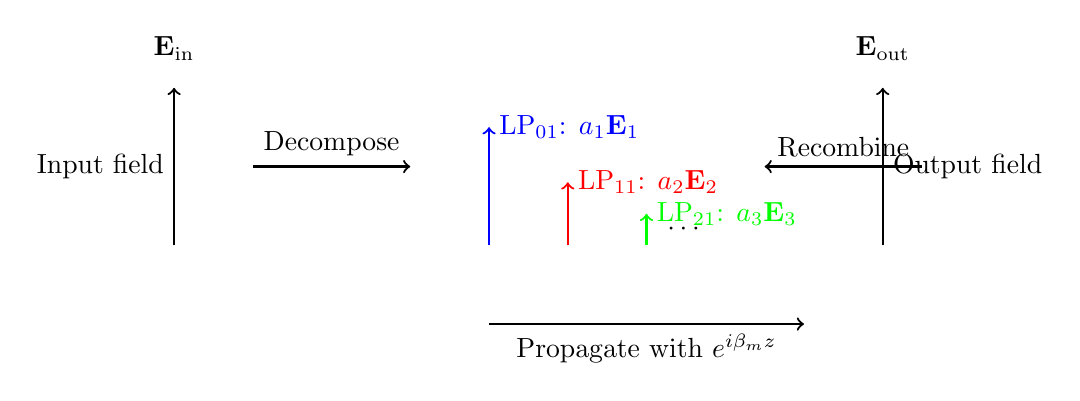
\begin{tikzpicture}
% Input field
\draw[thick, ->] (0,0) -- (0,2) node[midway, left] {Input field};
\draw[thick] (0,2.5) node {$\mathbf{E}_{\text{in}}$};

% Decomposition arrow
\draw[thick, ->] (1,1) -- (3,1) node[midway, above] {Decompose};

% Modes
\draw[thick, blue, ->] (4,0) -- (4,1.5) node[right] {LP$_{01}$: $a_1 \mathbf{E}_1$};
\draw[thick, red, ->] (5,0) -- (5,0.8) node[right] {LP$_{11}$: $a_2 \mathbf{E}_2$};
\draw[thick, green, ->] (6,0) -- (6,0.4) node[right] {LP$_{21}$: $a_3 \mathbf{E}_3$};
\draw (6.5, 0.2) node {$\cdots$};

% Propagation
\draw[thick, ->] (4,-1) -- (8,-1) node[midway, below] {Propagate with $e^{i\beta_m z}$};

% Output
\draw[thick, ->] (9,0) -- (9,2) node[midway, right] {Output field};
\draw[thick] (9,2.5) node {$\mathbf{E}_{\text{out}}$};

% Recombination
\draw[thick, <-] (7.5,1) -- (9.5,1) node[midway, above] {Recombine};
\end{tikzpicture}
\end{center}

\section{Example: Single-Mode Fiber}

For a single-mode fiber (V < 2.405), only the LP$_{01}$ mode propagates.

\textbf{Modal expansion simplifies to:}
\begin{equation}
\mathbf{E}(\rho, \phi, z, t) = a_{01} \mathbf{E}_{01}(\rho, \phi) e^{i\beta_{01} z} e^{-\alpha z/2} e^{-i\omega t} + \text{c.c.}
\end{equation}

This is \textbf{much simpler} than the full Helmholtz equation solution!

\section{Comparison: Different Approaches}

\begin{center}
\begin{tabular}{|p{0.45\textwidth}|p{0.45\textwidth}|}
\hline
\textbf{Direct PDE Solution} & \textbf{Modal Expansion} \\
\hline
Solve full 3D Helmholtz equation & Reduce to 2D eigenvalue problem \\
\hline
Difficult with boundary conditions & Modes automatically satisfy BC \\
\hline
No physical insight & Clear mode picture \\
\hline
Coupling between components & Modes propagate independently \\
\hline
Hard to generalize & Easy to add dispersion, loss \\
\hline
\end{tabular}
\end{center}

\section{Connection to Quantum Field Theory}

In quantum field theory, we quantize \textbf{each mode separately}:
\begin{equation}
\hat{\mathbf{A}}(\rho, \phi, z) = \sum_m \sqrt{\frac{\hbar\omega_m}{2\epsilon_0 \epsilon_m V_m}} \left[\hat{a}_m \mathbf{E}_m(\rho, \phi) e^{i\beta_m z} + \text{h.c.}\right]
\end{equation}

Each mode becomes an independent quantum harmonic oscillator!

\section{Key Formulas Summary}

\begin{align}
\text{Modal expansion:} \quad & \mathbf{E} = \sum_m a_m \mathbf{E}_m(\rho,\phi) e^{i(\beta_m z - \omega t)} \\[0.3cm]
\text{Eigenvalue equation:} \quad & \nabla_\perp^2 \mathbf{E}_m + (k_0^2 n^2 - \beta_m^2)\mathbf{E}_m = 0 \\[0.3cm]
\text{Characteristic equation:} \quad & \frac{uJ_1(u)}{J_0(u)} = \frac{wK_1(w)}{K_0(w)}, \quad u^2 + w^2 = V^2 \\[0.3cm]
\text{Mode amplitude:} \quad & a_m = \frac{1}{N_m}\int \mathbf{E}_{\text{in}} \cdot \mathbf{E}_m^* \, dA \\[0.3cm]
\text{Orthogonality:} \quad & \int \mathbf{E}_m^* \cdot \mathbf{E}_n \, dA = N_m \delta_{mn}
\end{align}

\section{Why Modal Expansion is Powerful}

\begin{enumerate}
\item \textbf{Reduces complexity}: 3D problem $\to$ sum of 2D problems
\item \textbf{Physical insight}: Each mode has clear properties ($\beta_m$, dispersion, loss)
\item \textbf{Independent propagation}: Modes don't couple (in linear regime)
\item \textbf{Easy to include effects}: Add dispersion via $\beta_m(\omega)$, loss via $\alpha_m$
\item \textbf{Measurement interpretation}: Detectors couple to specific modes
\item \textbf{Quantum ready}: Each mode $\to$ quantum oscillator
\end{enumerate}

\end{document}